% 03-eksperimentalni-postav.tex — Experimental setup (TASK §F.4).
\section{Eksperimentalni postav}
\label{sec:postav}

\subsection{Hardver i mreža}

Robot je \textbf{Universal Robots UR3e} s upravljačkom jedinicom PolyScope
5.9.5, u načinu rada \emph{Remote Control}, koji e-Series traži da bi prihvatio
vanjske RTDE naredbe. Praćenje pokreta izvodi \textbf{OptiTrack} sa softverom
Motive 3.0.1 i protokolom NatNet 4.0 pri 120 Hz. Robot, sustav Motive i
upravljačko računalo dijele mrežu 192.168.40.0/24, a tok podataka ide unicastom,
jer multicast kroz mrežnu opremu laboratorija nije prolazio.

Operater nosi usku sportsku majicu i rukavicu, na koje je zalijepljeno po pet
reflektirajućih markera za nadlakticu, podlakticu i šaku
(slika~\ref{fig:postav}). Svaki je skup u sustavu Motive definiran kao kruto
tijelo, premda markeri na tijelu nisu međusobno kruto vezani --- posljedicu tog
izbora vraćamo u poglavlju~\ref{sec:rasprava}. Prije mjerenja provedena je
kalibracija osi iz šest izoliranih pokreta, kojom su određeni Eulerova sekvenca,
indeks i predznak za svaki kanal. Robot se prije svakog pokusa vraća u
referentnu pozu, ekvivalent ispružene ruke, kako bi svi pokusi počinjali iz
istog stanja.

\begin{figure}[htbp]
  \centering
  \IfFileExists{figures/setup_photo.jpg}{%
    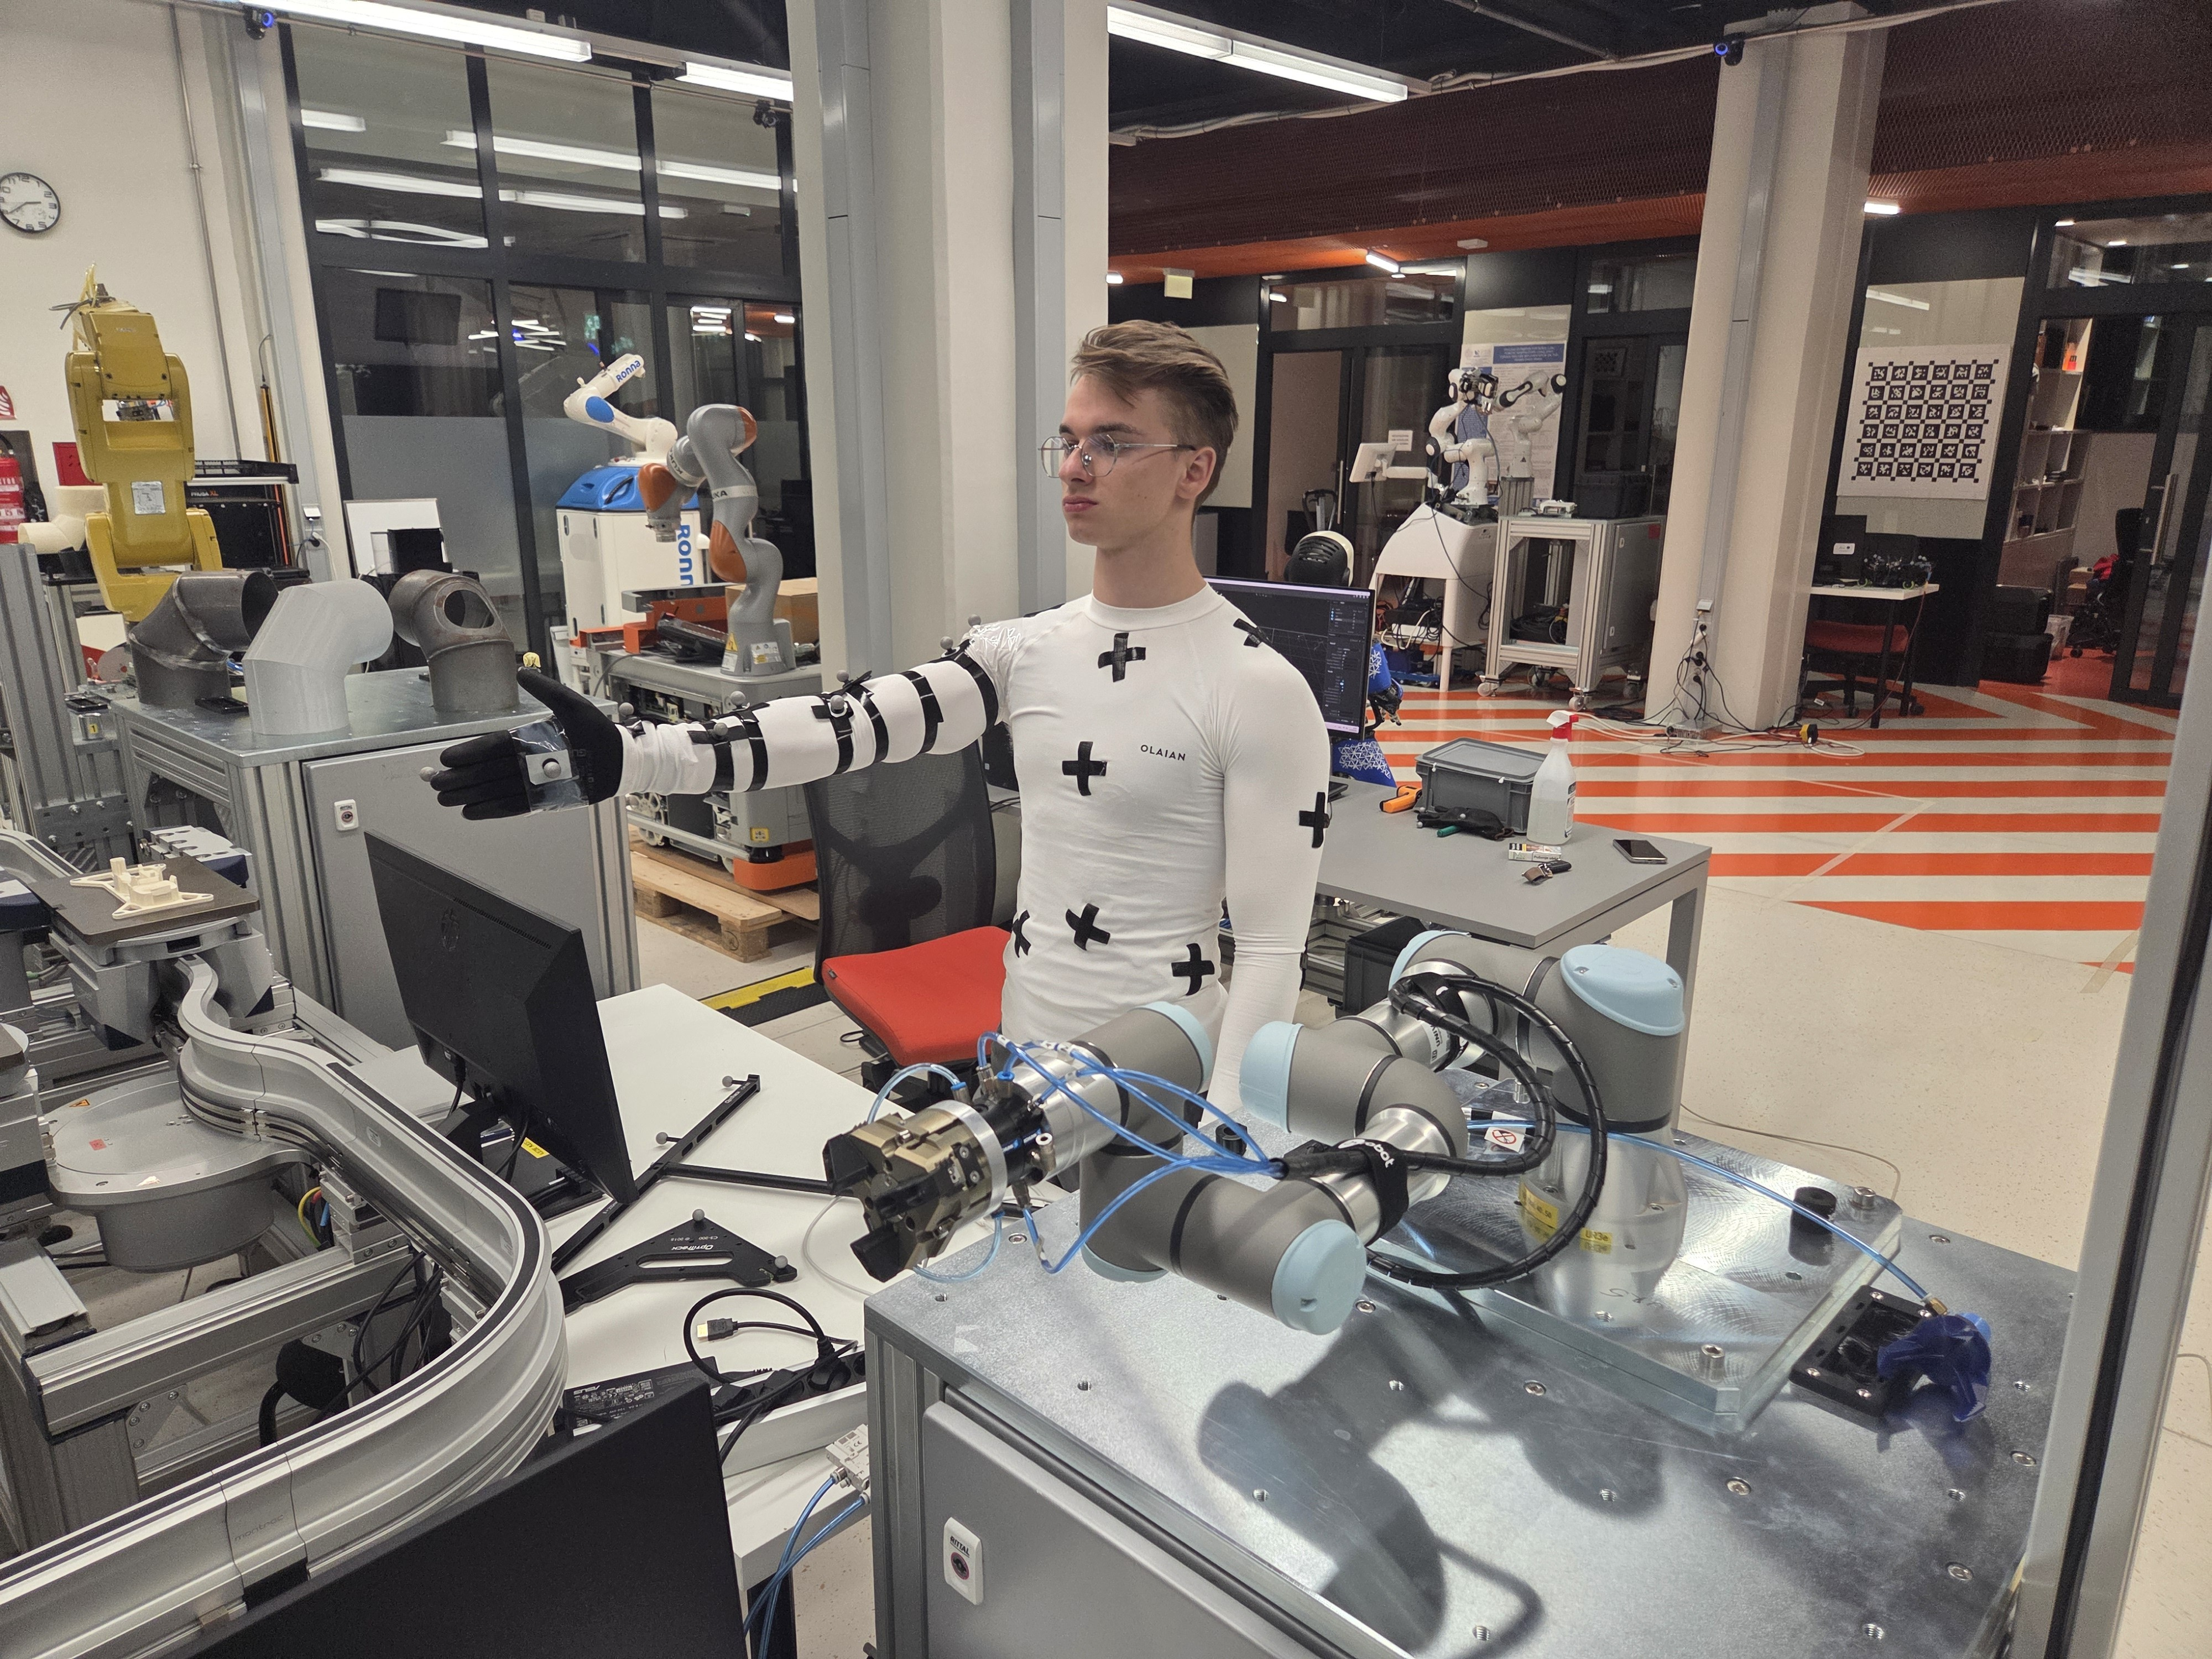
\includegraphics[width=\columnwidth]{figures/setup_photo.jpg}}{%
    \fbox{\parbox[c][3.2cm][c]{0.9\columnwidth}{\centering Fotografija postava}}}
  \caption{Operater i robot UR3e u zajedničkom radnom prostoru. Tri skupa
  markera --- nadlaktica, podlaktica, šaka --- daju šest zglobnih kanala.}
  \label{fig:postav}
\end{figure}

\subsection{Puštanje u rad na simulatoru}

Cijeli je obradni lanac prvo doveden u rad na simulatoru URSim. Ondje su
provjereni takt upravljačke petlje, preslikavanje kanala na zglobove, smjerovi i
pojačanja iz jednadžbe~(\ref{eq:mapiranje}) te djelovanje svakog sigurnosnog
sloja, uključujući ponašanje pri namjerno prekinutom toku podataka. Simulator je
za to prikladan jer omogućuje pogreške bez posljedica, budući da pogrešan predznak ondje znači
neispravnu animaciju, a na stvarnom robotu nekontrolirani zamah. Prijelaz na
stvarni robot bio je promjena odredišta u konfiguraciji, bez ijedne izmjene u
jezgri lanca. Sva mjerenja u nastavku potječu sa stvarnog robota.

\subsection{Sigurnosni protokol}

Granice nisu birane da budu što veće nego da nesigurno ponašanje bude nemoguće
prije nego što ga operater stigne primijetiti. Brzina zgloba ograničena je na
60--150$^\circ$/s ovisno o zglobu, raspon na $\pm$60--90$^\circ$ oko referentne
poze, a signal stariji od 150 ms zaustavlja izlaz. U pokusima koji su ciljano
ispitivali pojedini sloj, granica je bila stegnuta na 25$^\circ$/s za ograničenje brzine
i $\pm$25$^\circ$ za ograničenje raspona, kako bi sloj sigurno okinuo unutar
raspona pokreta koji čovjek može izvesti.

Iznosi su provjereni PFL proračunom norme ISO/TS 15066 \cite{iso15066}, u kojoj se
najveća dopuštena relativna brzina računa kao $v_\text{rel,max} = F_\text{max}/\sqrt{\mu k}$
uz reduciranu masu $\mu$ sustava čovjek--robot \cite[str.~4]{ghanbarzadeh2025}. Za regiju
podlaktice i zapešća norma navodi $F_\text{max} = 160$~N, $k = 40$~N/mm i $m_H = 2$~kg. Uz
konzervativnu efektivnu masu robota $m_R = M/2 = 5{,}6$~kg za UR3e bez alata slijedi
$\mu = 1{,}47$~kg i prag $v_\text{rel,max} = 0{,}66$~m/s. Obodna brzina prirubnice pri
zadanim granicama iznosi 0,48 m/s na laktu (J3, 120$^\circ$/s), 0,53 m/s u bazi
(J1, 60$^\circ$/s) i ispod 0,14 m/s na zapešću, dakle unutar praga, pri čemu obvezni kanal
lakta ima rezervu faktora 1,4. Elevacija ramena (J2) sa 150$^\circ$/s daje 1,22 m/s zbog
najduljeg kraka, pa bi usklađenost pri punom dosegu ondje tražila 81$^\circ$/s.
Postav nema mjerenje udaljenosti čovjeka od robota, pa nema ni
prilagodbe brzine blizini kakvu predlaže dinamički SSM \cite[str.~1]{peng2025};
zaštita je zato namjerno konzervativna, jednaka u cijelom radnom prostoru.
Gumb za zaustavljanje u nuždi bio je cijelo vrijeme u dosegu operatera i
promatrača.

\subsection{Matrica pokusa}

Proveden je 21 pokus na stvarnom robotu (tablica~\ref{tab:matrica}) uz detaljno bilježenje telemetrije i sinkroniziranih videozapisa. Riječ je o 21 različitom ispitnom scenariju, a ne o ponavljanjima istog uvjeta. Svi pokusi rade u načinu sa šest stupnjeva slobode, pri čemu kut lakta u svakom pokusu vodi zglob J3, pa obvezno preslikavanje raspolaže eksperimentalnim podacima kroz sve izvedene testove.

\begin{table}[H]
  \caption{Matrica pokusa. Sve mjereno na stvarnom robotu UR3e.}
  \label{tab:matrica}
  \centering\small
  \begin{tabularx}{\columnwidth}{l X r}
    \hline
    \textbf{Oznaka} & \textbf{Sadržaj} & \textbf{Broj} \\
    \hline
    T1a, T1b   & vjernost oponašanja (prirodni tempo i prolaz po zglobovima) & 2 \\
    T2a--T2d   & usporedba četiriju filtara na robotu & 4 \\
    T3a--T3d   & sigurnosni slojevi i zaustavljanje u nuždi & 4 \\
    T4a--T4e   & dodano kašnjenje 0--400 ms & 5 \\
    T5a--T5e   & ispitivanje gubitka paketa (0--30\,\%) & 5 \\
    T6         & dinamika pri naglim pokretima & 1 \\
    \hline
    \multicolumn{2}{l}{\textbf{Ukupno}} & \textbf{21} \\
    \hline
  \end{tabularx}
\end{table}

Uz teleometriju je zabilježen sinkronizirani dualni videozapis svakog pokusa pri čemu je vanjskom kamerom snimljena fizička reakcija operatera i robota, dok je snimkom zaslona zabilježeno 3D praćenje unutar programskog paketa Motive.

\subsection{Programska provjera}

Obradni lanac pokriven je s 79 automatiziranih testova (\texttt{pytest}) koji
provjeravaju kinematiku, filtre, protokol, sigurnosni sloj, zapisivanje kutova i
integraciju cijele petlje na sintetičkom izvoru. Prolaz svih testova bio je
uvjet za svaku promjenu koda koja je prethodila mjerenju.

\FloatBarrier
